\section{Absorption models and the method of characteristics}
\label{sec:moc}

Birth--death dynamics of pathogenic particles inside a host cell that can rupture leave open the question of what happens when several hosts share a medium and the first cell ruptures. Immediate transfer of the entire intracellular load into another host is a strong modelling assumption. A more realistic alternative is an \emph{absorption period}: following rupture, absorption events redistribute the released cohort among remaining hosts before intracellular birth, death, and rupture resume. Working towards such models, we begin with a pathogenic cohort infiltrating a single host cell.

Three models are treated in increasing order of difficulty. In the first two, particles are conserved or only lost, the state space is finite, and independence delivers the generating function without solving a partial differential equation. In the third, intracellular replication opens an infinite state space, the independence shortcut fails as a computational device, and the PDE must be solved by the method of characteristics. Characteristics are first tested on absorption--death, where the answer is already known, and then applied to absorption--birth--death.

\subsection{Absorption only}
\label{sec:absonly}

The simplest process has a single host that absorbs particles, with no birth or death of pathogen within the host. Let \(\xt\) and \(\yt\) denote intracellular and extracellular counts. Inter-event times are exponential, so \(\{(\xt,\yt):t\ge0\}\) is a continuous-time Markov chain.

Over an infinitesimal interval \(\Delta t\),
\begin{align*}
     \pr{\Delta\xx= 1,\;\Delta\yy = -1 \;|\; \yt = j} &= j \alpha \Delta t,  &&\text{(absorption)}\\
     \pr{\Delta\xx= 0,\;\Delta\yy = 0 \;|\; \yt = j} &= 1 -  j \alpha \Delta t,  &&\text{(no event)}
\end{align*}
with initial condition \(\xx_0=0\), \(\yy_0=N\). Writing \(\pt=\pr{\xt=i,\ \yt=j}\), the forward Kolmogorov equations are
\begin{equation}
\label{F1}
\ddt{\p} = \alpha(j+1)p_{i-1,j+1} - \alpha j\,\p .
\end{equation}
With the generating function
\begin{equation}
\label{pgfDef}
G(x,y,t) = \sum_i\sum_j \pt\, x^iy^j
=\mean{x^{\xt}y^{\yt}},
\end{equation}
multiplying \cref{F1} by \(x^iy^j\), summing, and rearranging produces the first-order PDE
\begin{equation}
\label{PDE1}
\pddt{G(x,y,t)} = \alpha\left(x - y\right) \pdd{G(x,y,t)}{y},
\qquad G(x,y,0) = y^N .
\end{equation}
Particles are neither created nor destroyed, so \(\pt=0\) whenever \(i+j\neq N\).

\subsubsection*{Exploiting independence}

Define more generally
\begin{equation*}
G_n(x,y,t) = \sum_i\sum_j \pr{\xt = i,\;\yt=j \;|\;\xx_0 = 0,\;\yy_0=n } x^i y^j .
\end{equation*}
In pure absorption the \(n\) particles move independently, so
\begin{equation}
\label{indRelPGF}
G_n(x,y,t) = \bigl(G_1(x,y,t)\bigr)^n .
\end{equation}
For a single particle, the only reachable states have \(i+j=1\), and
\begin{align*}
p_{0,1}(t) = \ee^{-\alpha t}, && p_{1,0}(t) = 1 - \ee^{-\alpha t} .
\end{align*}

\begin{figure}[H]
\centering
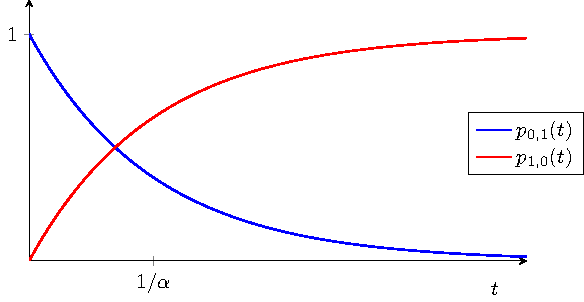
\includegraphics[width = 0.62\textwidth]{figures/IMG_ch3/abs1.pdf}
\caption{Single-particle absorption-only state probabilities: \(p_{0,1}\) decays exponentially at rate \(\alpha\); \(p_{1,0}\) rises to one.}
\label{fig:abs1}
\end{figure}

Hence
\begin{equation*}
G_1(x,y,t) = \lrb{1-\ee^{-\alpha t}}x + \ee^{-\alpha t}y ,
\end{equation*}
and
\begin{equation}
\label{eq:Gabsonly}
G_n(x,y,t) = \Bigl(\lrb{1-\ee^{-\alpha t}}x + \ee^{-\alpha t}y\Bigr)^n .
\end{equation}
This satisfies \cref{PDE1} with \(G_n(x,y,0)=y^n\). Equivalently, \(\xt\sim\mathrm{Binomial}(n,1-\ee^{-\alpha t})\).

\subsection{Absorption--death}
\label{sec:absdeath}

A particle inside the host may die. Transitions become
\begin{align*}
     \pr{\Delta\xx= 1,\;\Delta\yy = -1 \;|\; \yt = j} &= j \alpha \Delta t,  &&\text{(absorption)}\\
      \pr{\Delta\xx= -1,\;\Delta\yy = 0 \;|\; \xt = i} &= i \mu \Delta t,  &&\text{(death)}\\
     \pr{\Delta\xx= 0,\;\Delta\yy = 0 \;|\; \yt = j,\, \xt=i} &= 1 -  \lrb{ j\alpha + i\mu}\Delta t,
\end{align*}
with forward equations
\begin{equation}
\label{FK1}
\ddt{\p} = \alpha(j+1)p_{i-1,j+1} + \mu(i+1)p_{i+1,j} - (\alpha j + \mu i)\p
\end{equation}
and generating-function PDE
\begin{equation}
\label{PDE2}
\pddt{G(x,y,t)} = \mu(1-x)\pdd{G(x,y,t)}{x} + \alpha\left(x - y\right)\pdd{G(x,y,t)}{y},
\qquad G(x,y,0)=y^N.
\end{equation}
Independence still holds. For one particle,
\begin{align}
\label{eq:absdeathstates}
p_{0,1}(t) = \ee^{-\alpha t}, &&
p_{1,0}(t) = \frac{\alpha}{\mu - \alpha}\Bigl(\ee^{-\alpha t} - \ee^{-\mu t}\Bigr), &&
p_{0,0}(t) = 1 - p_{0,1}(t) - p_{1,0}(t).
\end{align}

\begin{figure}[H]
\centering
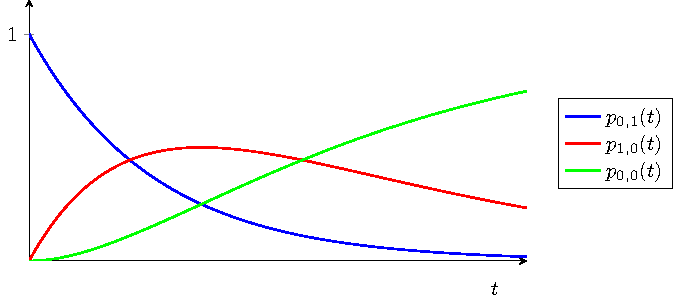
\includegraphics[width = 0.62\textwidth]{figures/IMG_ch3/abs2.pdf}
\caption{Single-particle absorption--death probabilities: outside (blue), inside (red), dead (green).}
\label{fig:abs2}
\end{figure}

The general generating function is
\begin{equation}
\label{eq:Gabsdeath}
G_n(x,y,t) = \Bigl(1-\tfrac{\mu}{\mu - \alpha}\ee^{-\alpha t} + \tfrac{\alpha}{\mu - \alpha}\ee^{-\mu t}
+ \tfrac{\alpha}{\mu - \alpha}\bigl(\ee^{-\alpha t} - \ee^{-\mu t}\bigr)x + \ee^{-\alpha t}y\Bigr)^n .
\end{equation}

\subsection{The method of characteristics, tested on absorption--death}
\label{sec:mocabsdeath}

Before treating absorption--birth--death, where independence no longer yields a finite closed form for \(G_1\), we re-derive \cref{eq:Gabsdeath} from the PDE by characteristics, as a controlled test.\footnote{I am grateful to Benjamin Sharp for advice on applying the method of characteristics to three-variate problems that unlocked this development.}

Introduce \((x,y,t)\to(s,r,\tau)\) with \(G\) regarded as a function of \(\tau\) alone along characteristics of constant \(s,r\). The initial surface is
\begin{equation}
\label{ICpar}
x(s,r,0) = s, \qquad y(s,r,0) = r, \qquad t(s,r,0) = 0 .
\end{equation}
Comparing the chain rule for \(\mathrm{d}G/\mathrm{d}\tau\) with \cref{PDE2} written as
\begin{equation*}
0 = -\pddt{G} + \mu(1-x)\pdd{G}{x} + \alpha(x-y)\pdd{G}{y}
\end{equation*}
produces the characteristic system
\begin{align}
\dda{G}{\tau} &= 0, \label{ch11}\\
\dda{t}{\tau} &= -1, \label{ch12}\\
\dda{x}{\tau} &= \mu(1-x), \label{ch13}\\
\dda{y}{\tau} &= \alpha(x-y). \label{ch14}
\end{align}

\paragraph{The equation for \(G\), \eqref{ch11}.}
\(G\) is constant along characteristics. With \(G(s,r,0)=r^N\),
\begin{equation}
\label{GrN}
G(s,r,\tau) = r^N .
\end{equation}
The problem reduces to expressing \(r\) in terms of \((x,y,t)\).

\paragraph{The equation for \(t\), \eqref{ch12}.}
\begin{equation}
\label{minustau}
t = -\tau .
\end{equation}
The characteristic parameter runs backwards in time, so the initial surface is reachable from any \((x,y,t)\).

\paragraph{The equation for \(x\), \eqref{ch13}.}
\begin{equation}
\label{sandxwithtau}
1-x = (1-s)\ee^{-\mu\tau} .
\end{equation}

\paragraph{The equation for \(y\), \eqref{ch14}.}
Solving with integrating factor \(\ee^{\alpha\tau}\) and imposing \cref{ICpar} yields
\begin{equation}
\label{ywithr1}
y = 1 - \frac{\alpha}{\alpha-\mu}(1-s)\ee^{-\mu\tau} + \lrb{r + \frac{\alpha}{\alpha-\mu}(1-s) - 1}\ee^{-\alpha\tau}.
\end{equation}

\paragraph{Recovering the solution.}
Solving \cref{ywithr1} for \(r\), substituting \(s\) from \cref{sandxwithtau} and \(\tau=-t\), and applying \cref{GrN} reproduces \cref{eq:Gabsdeath} exactly. The two routes agree; the machinery is ready for the case where only one is available.

\subsection{Absorption--birth--death}
\label{sec:absbirthdeath}

With intracellular replication, infinitely many states are reachable from a single particle, so \(G_1\) is an infinite series and factorisation no longer simplifies the computation. The PDE must be solved directly.

Transitions:
\begin{align*}
     \pr{\Delta\xx= 1,\;\Delta\yy = -1 \;|\; \yt = j} &= j \alpha \Delta t,  &&\text{(absorption)}\\
     \pr{\Delta\xx= 1,\;\Delta\yy = 0 \;|\; \xt = i} &= i \beta \Delta t,  &&\text{(birth)}\\
      \pr{\Delta\xx= -1,\;\Delta\yy = 0 \;|\; \xt = i} &= i \mu \Delta t,  &&\text{(death)}\\
     \pr{\Delta\xx= 0,\;\Delta\yy = 0 \;|\; \yt = j,\, \xt=i} &= 1 -  \lrb{ j\alpha + i\mu + i\beta}\Delta t,
\end{align*}
with forward equation
\begin{equation}
\label{FK3}
\pddt{\p} = \alpha(j+1)p_{i-1,j+1} + \mu(i+1)p_{i+1,j} + \beta(i-1)p_{i-1,j} - (\alpha j + \mu i + \beta i)\p
\end{equation}
and generating-function PDE
\begin{equation}
\label{PDE3}
\pddt{G} = \lrb{\mu - (\mu+\beta)x + \beta x^2}\pdd{G}{x} + \alpha(x-y)\pdd{G}{y},
\qquad G(x,y,0) = y^N .
\end{equation}
The characteristic system is
\begin{align}
\dda{G}{\tau} &= 0, \label{ch21}\\
\dda{t}{\tau} &= -1, \label{ch22}\\
\dda{x}{\tau} &= \mu-(\mu+\beta)x + \beta x^2, \label{ch23}\\
\dda{y}{\tau} &= \alpha(x-y), \label{ch24}
\end{align}
with initial surface \cref{ICpar}.

\paragraph{The equations for \(G\) and \(t\), \eqref{ch21}--\eqref{ch22}.}
\begin{equation}
\label{gngngn}
G(s,r,\tau) = r^N,
\qquad t = -\tau .
\end{equation}

\paragraph{The equation for \(x\), \eqref{ch23}.}
The right-hand side is Riccati and factorises as
\begin{equation}
\label{eq:xpm}
\mu - (\mu+\beta)x + \beta x^2 = \beta(x-x_+)(x-x_-),
\qquad
x_+ = 1,\quad x_- = \frac{\mu}{\beta}.
\end{equation}
Write \(b_1=\beta-\mu\) for the net intracellular growth rate. Separating variables and applying \cref{ICpar} gives
\begin{equation}
\label{eq:xratio}
\frac{x-x_+}{x-x_-} = \lrb{\frac{s-x_+}{s-x_-}}\ee^{b_1\tau},
\end{equation}
or
\begin{equation}
\label{xabd}
x(\tau) = \frac{x_+(s-x_-) - x_-(s-x_+)\ee^{b_1\tau}}{(s-x_-) - (s-x_+)\ee^{b_1\tau}} .
\end{equation}

\paragraph{The equation for \(y\), \eqref{ch24}.}
With integrating factor,
\begin{equation}
\label{eq:yint}
\dda{}{\tau}\lrb{\ee^{\alpha\tau}y} = \alpha\,\ee^{\alpha\tau}x(\tau).
\end{equation}
Expanding \(x(\tau)\) as a geometric series in
\begin{equation*}
\zeta(\tau) = \lrb{\frac{s-x_+}{s-x_-}}\ee^{b_1\tau}
\end{equation*}
yields term-by-term integrals and defines
\begin{equation}
\label{eq:Psidef}
\Psi(\zeta) \;=\; x_+ + \frac{\alpha}{\beta}\sum_{n=1}^{\infty}\frac{\zeta^{\,n}}{n+\delta},
\qquad \delta = \frac{\alpha}{b_1} = \frac{\alpha}{\beta-\mu}.
\end{equation}
Imposing the initial condition for \(y\) and restoring \((x,y,t)\) produces the closed form.

\begin{proposition}[Generating function for absorption--birth--death]
\label{prop:Gabd}
With \(x_+=1\), \(x_-=\mu/\beta\), \(b_1 = \beta-\mu\), \(\delta = \alpha/b_1\),
\(W = (x-x_+)/(x-x_-)\) and \(\Psi\) as in \cref{eq:Psidef},
\begin{equation}
\label{eq:Gabd}
\boxed{\;
G(x,y,t) = \Bigl\{\ee^{-\alpha t}\bigl[y - \Psi(W)\bigr] + \Psi\bigl(W\ee^{b_1 t}\bigr)\Bigr\}^{N}. \;}
\end{equation}
\end{proposition}

Three checks confirm the result. At \(t=0\) the \(\Psi\) terms cancel and \(G=y^N\). At \(x=y=1\), \(W=0\) and \(\Psi(0)=1\), so \(G=1\). Setting \(x=1\) alone gives
\begin{equation*}
G(1,y,t) = \bigl(\ee^{-\alpha t}y + 1 - \ee^{-\alpha t}\bigr)^N,
\end{equation*}
so \(\yt\sim\mathrm{Binomial}(N,\ee^{-\alpha t})\), as required by independent extracellular absorption. Beyond these, \cref{eq:Gabd} has been verified numerically against direct integration of \cref{FK3}, agreeing to around \(10^{-13}\) across sub- and supercritical intracellular regimes for \(N=1,2,3\).

\subsubsection*{Hypergeometric form}

The series in \cref{eq:Psidef} is a Gauss hypergeometric function. With the Pochhammer symbol \((q)_n\),
\begin{equation}
\label{eq:2F1def}
{}_2F_1(a,b;c;z) = \sum^\infty_{n=0}\frac{(a)_n(b)_n}{(c)_n}\frac{z^n}{n!},
\end{equation}
the case \(a=1\), \(b=\delta\), \(c=\delta+1\) collapses to
\begin{equation}
\label{eq:2F1simple}
{}_2F_1\lrb{1,\delta;\delta+1;z} = \sum_{n=0}^{\infty}\frac{\delta}{\delta+n}z^n ,
\end{equation}
and
\begin{equation}
\label{eq:Psihyp}
\Psi(\zeta) = x_+ + (x_+-x_-)\Bigl[{}_2F_1\lrb{1,\delta;\delta+1;\zeta} - 1\Bigr].
\end{equation}
An alternative derivation of the same object via the integral \(\int\ee^{h\tau}/(p+q\ee^{k\tau})\,\mathrm{d}\tau\) is given in \cref{app:hyp}. Coefficient extraction from multilinear generating functions is recorded in \cref{app:extract}.

\begin{remark}[Domain of validity]
\label{rem:domain}
The series \cref{eq:Psidef} converges for \(|\zeta|<1\). In the subcritical intracellular regime \(\mu>\beta\), \(b_1<0\) and \(x_->1\), so for \(x\in[0,1]\) the arguments in \cref{eq:Gabd} lie in the unit disk. When \(\beta>\mu\) one uses the analytic continuation of \({}_2F_1\), for example the Euler integral representation.
\end{remark}

\begin{remark}[Resonance]
\label{rem:resonance}
Denominators in \cref{eq:Psidef} vanish when \(\alpha=n(\mu-\beta)\) for some integer \(n\ge1\). This is a removable resonance of the linearised \(y\)-equation; the generating function itself remains analytic in the parameters, and the corresponding term acquires a secular factor \(\tau\) in place of a pure exponential.
\end{remark}

\FloatBarrier
